\subsection{$90\degree$ Turn}

\subsubsection{Curved $90\degree$ Turn}

Figure \ref{fig:turns_cur_90deg_pos} and \ref{fig:turns_cur_90deg_camera} shows the optimized paths of a $90\degree$ path with varying turn radii. The results show that with a radius of $200$m, $150$m, and $50$m the optimization algorithm returns a smooth stable flight path. However, the camera position contains more nudges than for gentler turns, which happens because of the roll angle varying more. This can also be seen in Figure \ref{fig:turns_cur_90deg_roll}. When optimizing the turn with $50$m radius the roll angle reaches almost $30\degree$. It can also be seen that the sharper the turn the earlier the aircraft starts banking.

As expected the camera centre points deviates more from the original path than for gentler turns. After the $50$m radius turn in Figure \ref{fig:turns_cur_90deg_camera_50}, the camera position ends up with a significant deviance of $50$m away from the desired path. While this most likely would correct itself if the path was simulated further, it is a result of how the cost function is weighted. The weight on the camera position is very low compared to the weight put on control rates, as well as speed and altitude, which means that the deviance from the path has a smaller cost than correcting it.

A more surprising result is seen in Figures \ref{fig:turns_cur_90deg_camera_100} and \ref{fig:turns_cur_90deg_camera_100}. Even though the MPC is able to optimize the turn with $50$m radius, it is not able to return a stable flight path for the turn with $100$m radius. The camera position path is similar to previous failures: instead of optimizing the UAV position to track the camera path it uses the bank angle to achieve a satisfying short-term solution.

\begin{figure}
	\makebox[\textwidth][c]{
	\subfloat[$200$m][$200$m]{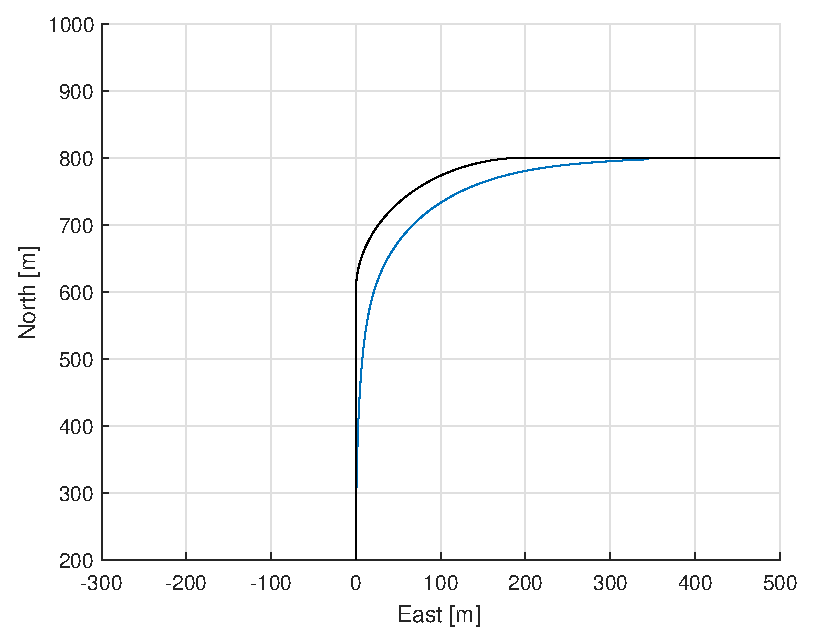
\includegraphics[width=0.5\textwidth, keepaspectratio=true]{../../results/opt/turns/curved/fig_90deg/uav_position_200m.eps}}
	\qquad
	\subfloat[$150$m][$150$m]{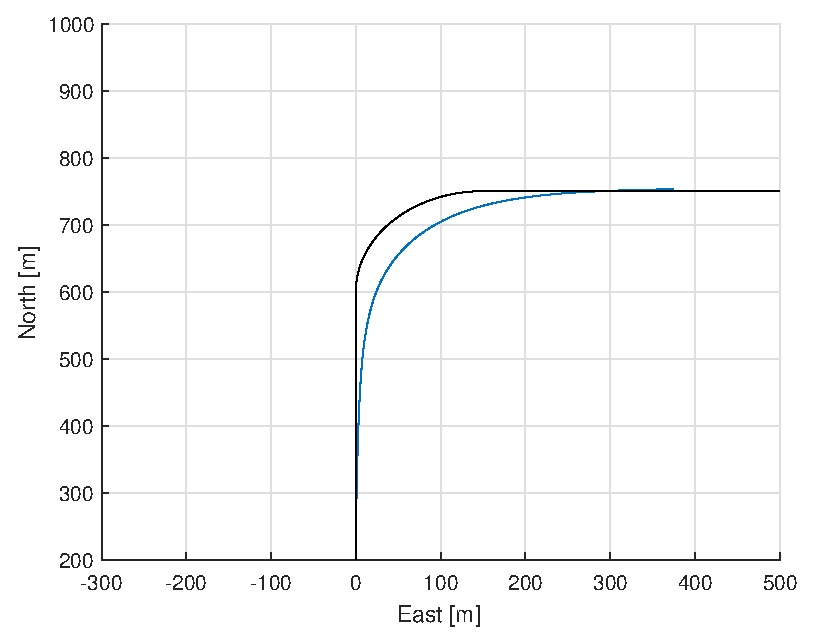
\includegraphics[width=0.5\textwidth, keepaspectratio=true]{../../results/opt/turns/curved/fig_90deg/uav_position_150m.eps}}}
	\makebox[\textwidth][c]{
	\subfloat[$100$m][$100$m]{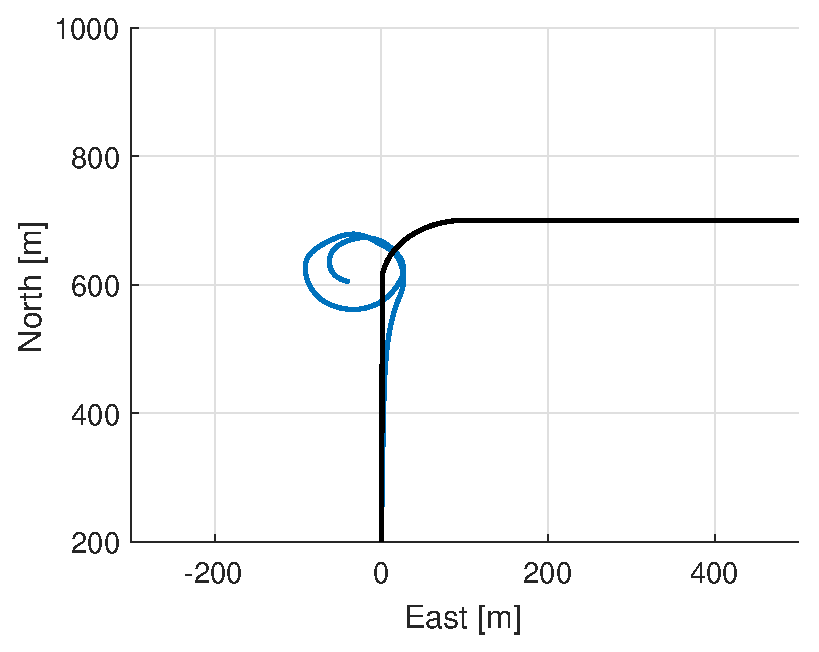
\includegraphics[width=0.5\textwidth, keepaspectratio=true]{../../results/opt/turns/curved/fig_90deg/uav_position_100m.eps}
	\label{fig:turns_cur_90deg_position_100}}
	\qquad
	\subfloat[$50$m][$50$m]{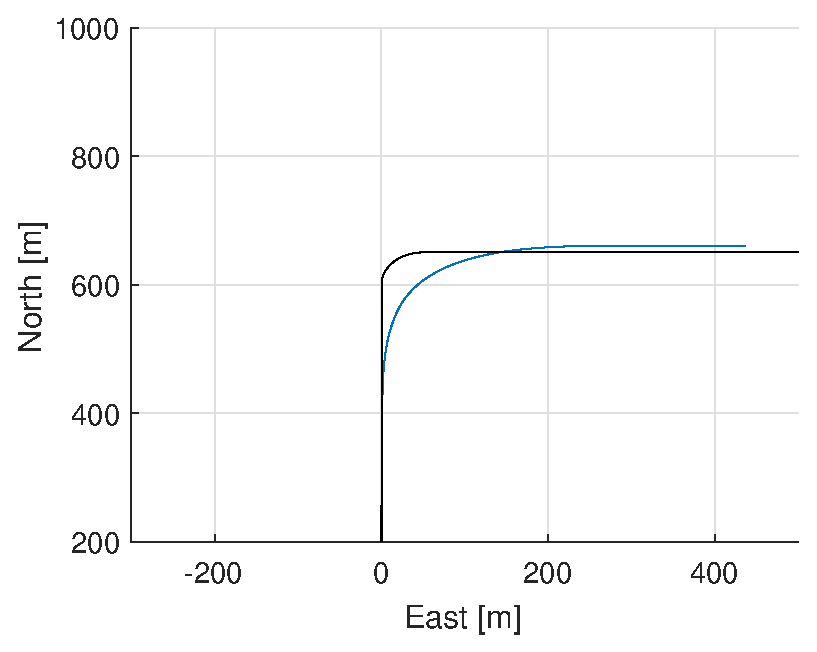
\includegraphics[width=0.5\textwidth, keepaspectratio=true]{../../results/opt/turns/curved/fig_90deg/uav_position_50m.eps}}}
	\caption{The position of the UAV when optimizing a curved $90\degree$ turn with varying radius.}
	\label{fig:turns_cur_90deg_pos}
\end{figure}

\begin{figure}
	\makebox[\textwidth][c]{
	\subfloat[$200$m][$200$m]{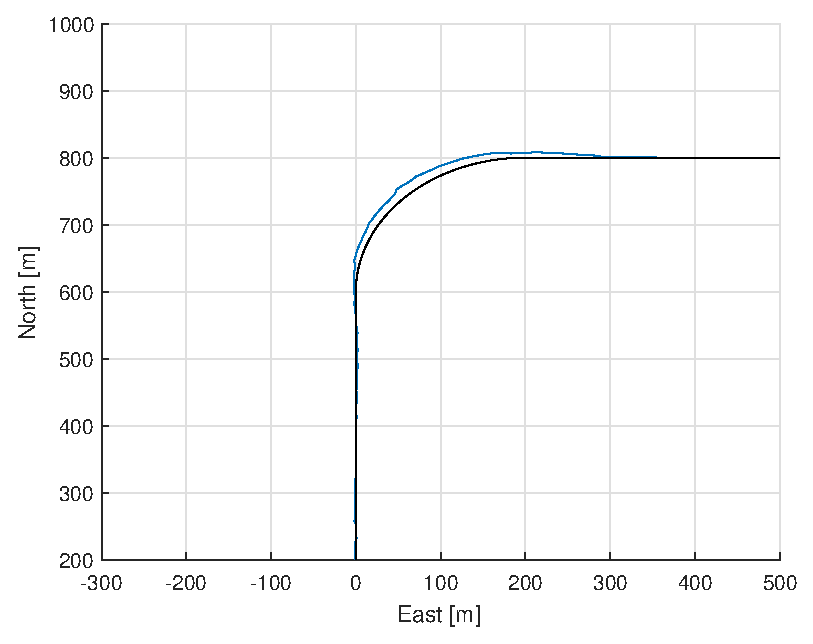
\includegraphics[width=0.5\textwidth, keepaspectratio=true]{../../results/opt/turns/curved/fig_90deg/camera_position_200m.eps}}
	\qquad
	\subfloat[$150$m][$150$m]{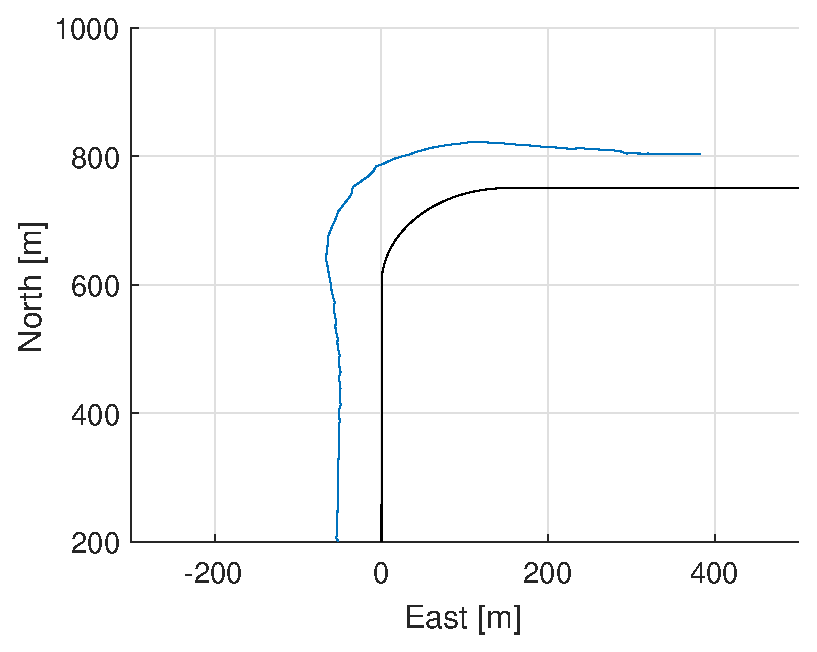
\includegraphics[width=0.5\textwidth, keepaspectratio=true]{../../results/opt/turns/curved/fig_90deg/camera_position_150m.eps}}}
	\makebox[\textwidth][c]{
	\subfloat[$100$m][$100$m]{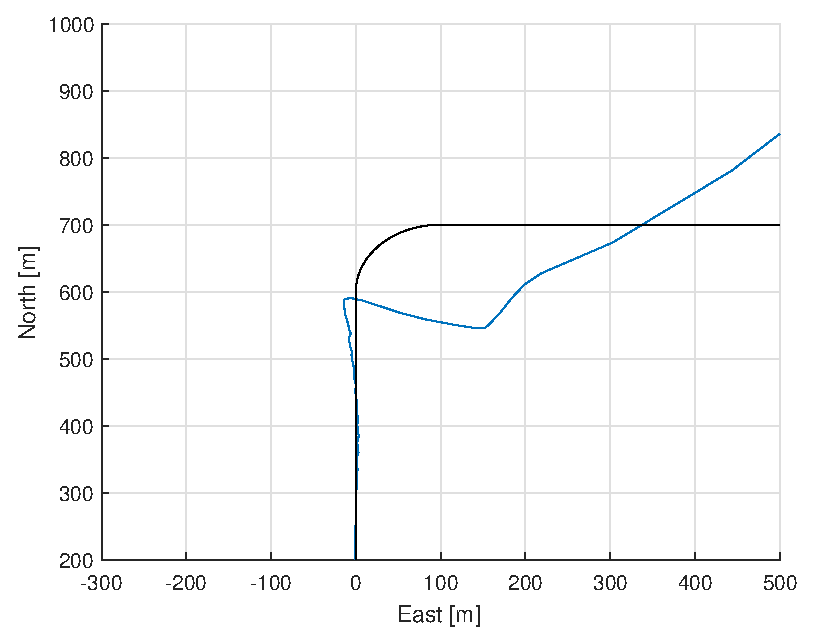
\includegraphics[width=0.5\textwidth, keepaspectratio=true]{../../results/opt/turns/curved/fig_90deg/camera_position_100m.eps}
	\label{fig:turns_cur_90deg_camera_100}}
	\qquad
	\subfloat[$50$m][$50$m]{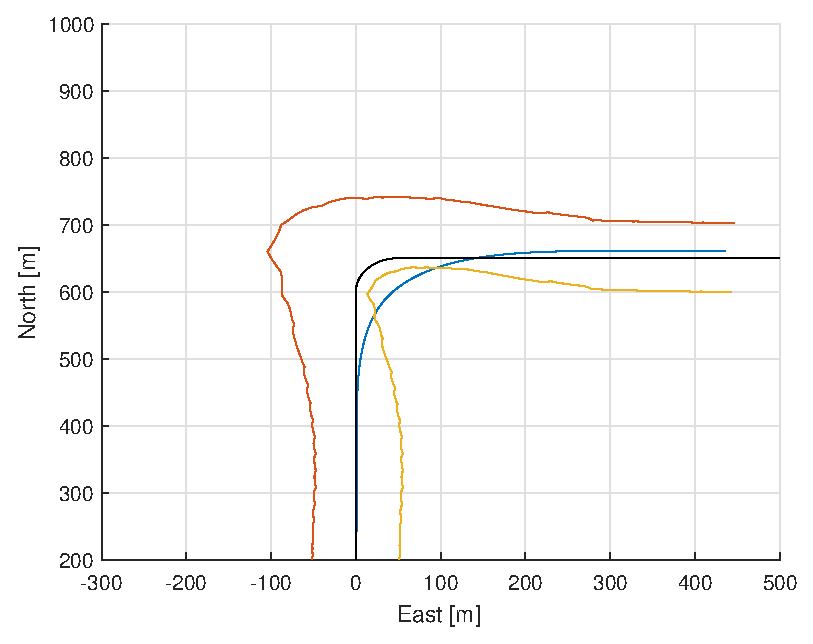
\includegraphics[width=0.5\textwidth, keepaspectratio=true]{../../results/opt/turns/curved/fig_90deg/camera_position_50m.eps}
	\label{fig:turns_cur_90deg_camera_50}}}
	\caption{The position of the camera when optimizing a curved $90\degree$ turn with varying radius.}
	\label{fig:turns_cur_90deg_camera}
\end{figure}

\begin{figure}
	\makebox[\textwidth][c]{
	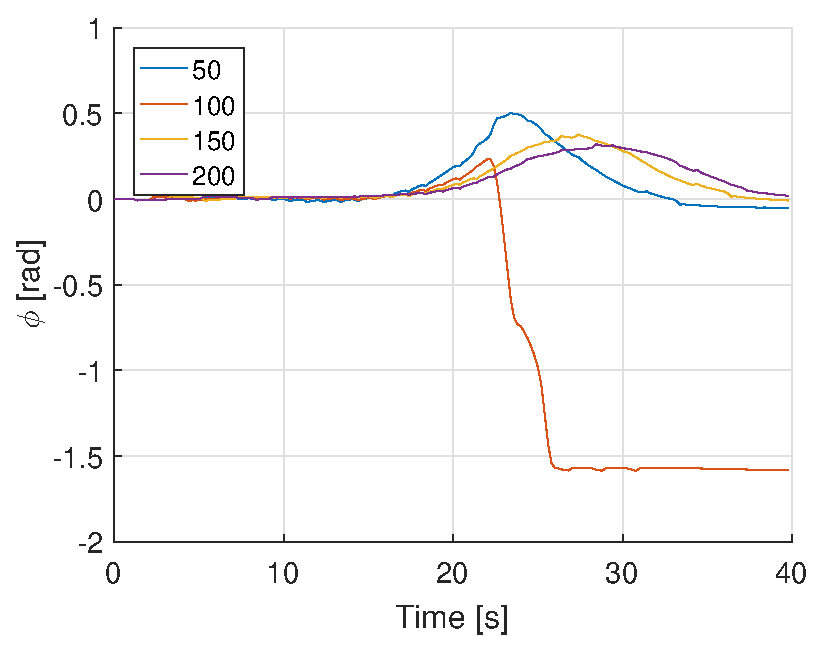
\includegraphics[width=0.8\textwidth, keepaspectratio=true]{../../results/opt/turns/curved/fig_90deg/attitude.eps}}
	\caption{The roll angle $\phi$ during the $90\degree$ turns.}
	\label{fig:turns_cur_90deg_roll}
\end{figure}


\subsubsection{Linear $90\degree$ Turn}

Since the MPC struggles to track a $70\degree$ corner, it is no surprise that it fails to track a $90\degree$ corner as seen in Figure \ref{fig:turns_lin_90deg}. Once again the MPC ends up with solving a difficult path using roll instead of the position, which ends with a bad solution. Different weightings on the position was tested without success.

\begin{figure}
	\makebox[\textwidth][c]{
	\subfloat[UAV position][UAV position.]{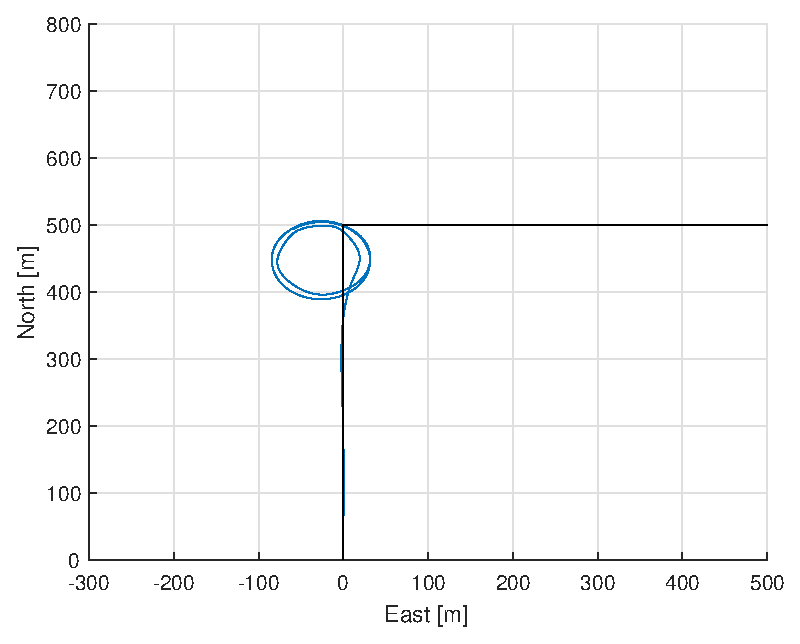
\includegraphics[width=0.5\textwidth, keepaspectratio=true]{../../results/opt/turns/linear/fig_90deg/uav_position.eps}}
	\qquad
	\subfloat[Camera position][Camera poistion.]{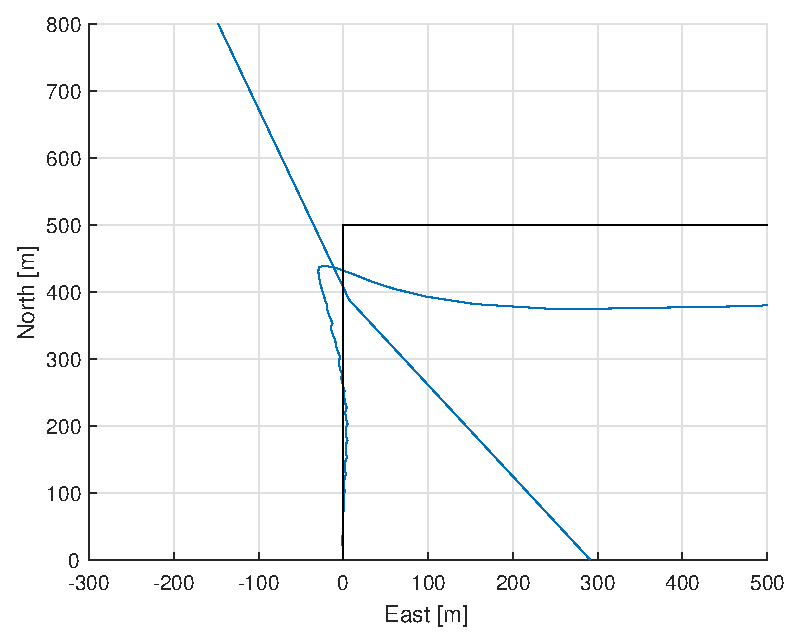
\includegraphics[width=0.5\textwidth, keepaspectratio=true]{../../results/opt/turns/linear/fig_90deg/camera_position.eps}}}
	\caption{Result of attempting to optimize a linear $90\degree$ turn.}
	\label{fig:turns_lin_90deg}
\end{figure}